Large language models suffer from several fundamental issues, which are not entirely solvable through training or prompt engineering. 
\citet{Gao.18.12.2023} stated that LLMs have significant limitations in knowledge-intesive or domain-specific tasks. Missing or unsufficient amount of information on a specific subject while training lead to wrong answers. For large language models this is called \textit{hallucinations} as defined in \citet{Huang.2023}. For retrieval-augmented generation systems (RAGs) the term hallucinations is defined for stating information without context. \citet{Rashkin.} defined hallucinations as any information that is neither inferable from nor stated by an external document. In this thesis I will use the definition for RAG systems. 

Factual wrong output from an LLM can have several reasons. The required information to answer this question can be private, stored on a database that is not accessible during training. Another reason might be that training or fine-tuning the model is expensive and thus done less frequent. Therefore the required information can be published more recently then the last training run. All those problems can be solved if the LLM is not used for the answer itself, but rather used for building a coherent text passage given a question and its answer. Then a database would store all relevant information and would be updated as frequent as required. At inference time the prompt is used to determine relevant chunks of documents within the database, which are then used for the generation of the answer.

This concept is very successful as \citet{Shuster.} showed. Factual wrong outputs are reduced and open-domain conversational capabilities are increased. \citet{Yu.2024} concluded that this improves the reliability and richnes of the produced content. \citet{Chen.2024} stated that external knowledge would be the key for resolving the above stated problems of LLMs, which make them more accurate and reliable.

There is a high variety in architectures and approaches for retrieval-augmented generation models. In this section, we will give an overview of the most common approaches and architectures and start with the most basic ones. The section will follow the definition of RAGs in \citet{Gao.18.12.2023} with naive RAGS, advanced RAGs, a modular architecture, and special cases. 

\subsection{Naive RAGs}
\label{sec:naive_rags}
Naive RAGs can be seen as the most basic form of a retrieval-augmented generation system. The core idea behind this concept is to give all relevant context for answering a question or solving a task into the prompt for the large language model. Then the LLM is only used for generating a coherent answer. Therefore it is required to ingest relevant data for the given use case beforehand. The system then retrieves relevant chunks or documents of this data at inference time. 


\begin{figure}[h!]
    \centering
    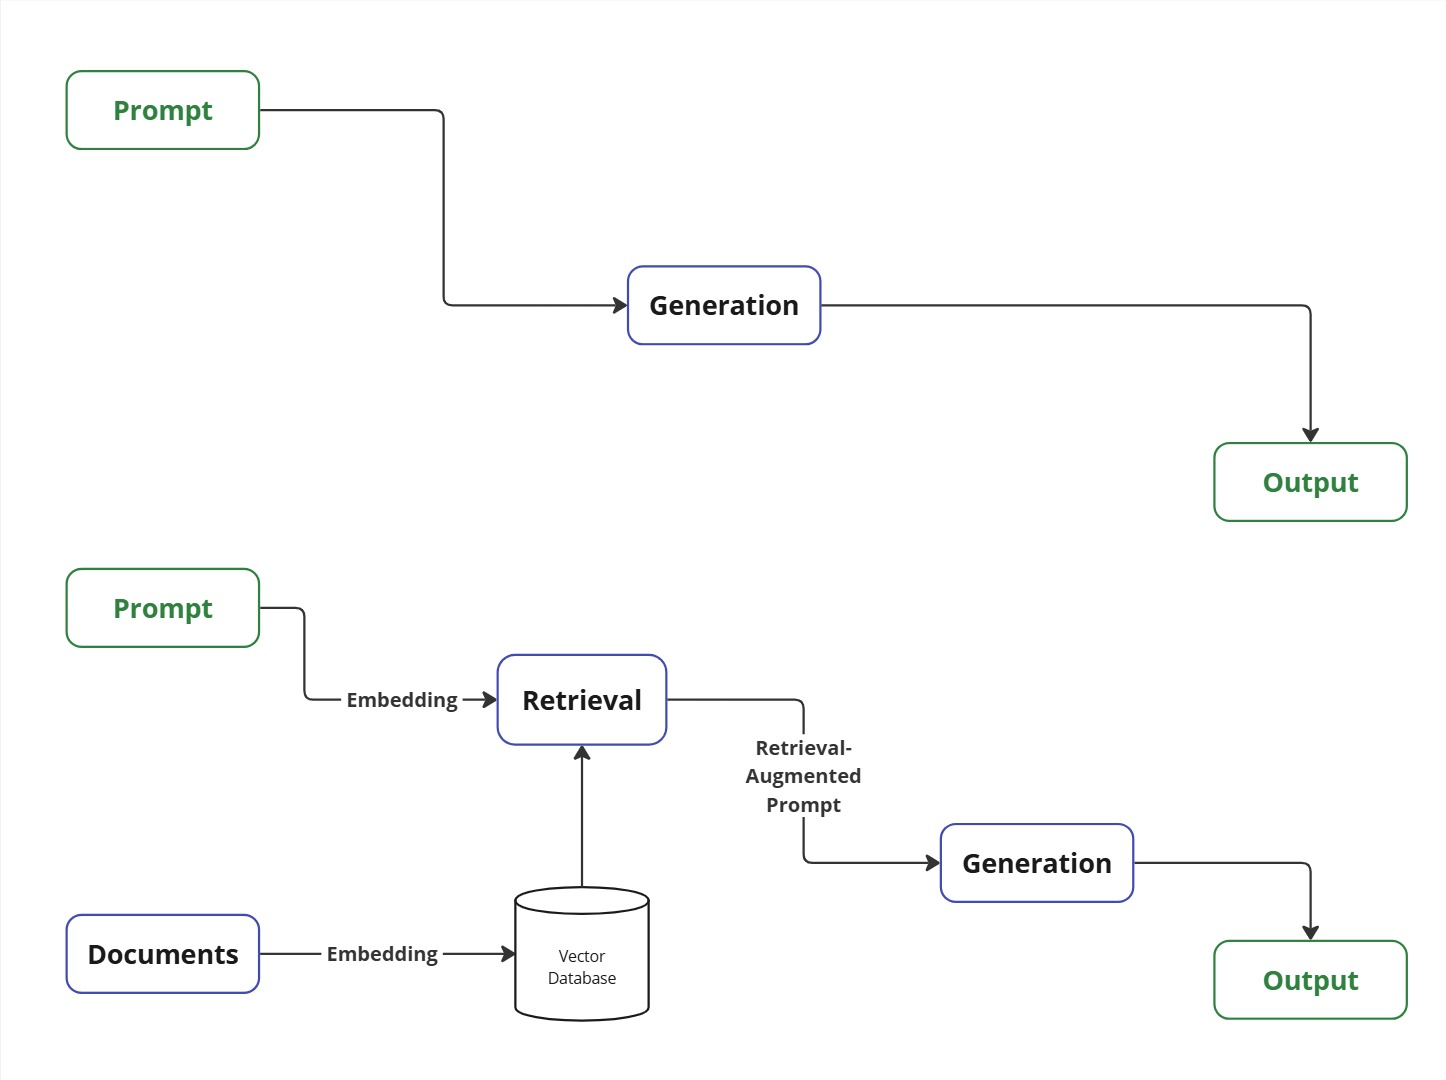
\includegraphics[width=0.75\textwidth]{images/LLM-vs-RAG.jpg}
    \caption{Comparison of the process to the prompt, above a standalone LLM that has a prompt and generate a response, below a RAG system that performs on a given set of documents and encoding or indexing and searchs for the most similar documents for a given prompt at inference time. Both prompt and documents are used for the generation process.}
    \label{fig:naive_rag}
\end{figure}

This procedure can be seen in figure \ref{fig:naive_rag}. In the literature the generation process is often refered as \textit{read}, because it reads the prompt and the provided context. In \citet{Gao.18.12.2023} they define the naive RAG system as \textit{Retrieve-Read}. The retrieval can be done with sparse retrieval (TF-IDF, BM25), dense retrieval (DPR) or a hybrid version as showed in section \ref{retrieval}. 

\citet{Gao.18.12.2023} listed several drawbacks for naive RAGs. The basic retrieval suffers from unsufficient recall and precision scores leading in irrelevant documents, missing context and bias. The integration of the provided context is a challenging process. The generator often overrelies on the augmented information, by just repeating the retrieved content and missing insightful conclusions. Therefore this simplistic form of RAG needs advanced techniques to overcome this issues. 

\subsection{Advanced RAGs}
\label{sec:advanced_rags}



\paragraph{Rewrite}
\label{sec:rewrite}

\paragraph{Rerank}
\label{sec:rerank}

\paragraph{Iterative RAGs}
\label{sec:iterative}

\paragraph{Recursive RAGs}
\label{sec:recursive}

\paragraph{Adaptive RAGs}
\label{sec:adaptive}

\subsection{General Modular RAG}
\label{sec:modular_rag}

\subsection{Special Cases}
\label{sec:special_cases}